\documentclass[11pt,a4paper,russian,intlimits]{ncc}
\usepackage[utf8]{inputenc}
\usepackage[T2A]{fontenc}
\DeclareUnicodeCharacter{2009}{\,}
\usepackage[margin=2cm]{geometry}

\usepackage{color}

\usepackage{hyperref}
\hypersetup{
    colorlinks=true,
    linkcolor=black,
    filecolor=magenta,
    urlcolor=cyan,
    linktoc=all,
}

\usepackage{graphicx}

% Needed for Asciidoc

\newcommand{\admonition}[2]{\textbf{#1}: {#2}}
\newcommand{\rolered}[1]{ \textcolor{red}{#1} }
\newcommand{\roleblue}[1]{ \textcolor{blue}{#1} }


\renewenvironment{quotation}
{   \leftskip 4em \begin{em} }
{\end{em}\par }

\def\signed#1{{\leavevmode\unskip\nobreak\hfil\penalty50\hskip2em
  \hbox{}\nobreak\hfil\raise-3pt\hbox{(#1)}%
  \parfillskip=0pt \finalhyphendemerits=0 \endgraf}}


\newsavebox\mybox

\newenvironment{aquote}[1]
  {\savebox\mybox{#1}\begin{quotation}}
  {\signed{\usebox\mybox}\end{quotation}}

\newenvironment{tquote}[1]
  {  {\bf #1} \begin{quotation} \\ }
  { \end{quotation} }

%% BOXES: http://tex.stackexchange.com/questions/83930/what-are-the-different-kinds-of-boxes-in-latex
%% ENVIRONMENTS: https://www.sharelatex.com/learn/Environments

\newenvironment{asciidocbox}
  {\leftskip6em\rightskip6em\par}
  {\par}

\newenvironment{titledasciidocbox}[1]
  {\leftskip6em\rightskip6em\par{\bf #1}\vskip-0.6em\par}
  {\par}



%%%%%%%%%%%%%%%%%%%%%%%%%%%%%%%%%%%%%%%%%%%%%%%%%%%%%%%%

%% http://texblog.org/tag/rightskip/


\newenvironment{preamble}
  {}
  {}

%% http://tex.stackexchange.com/questions/99809/box-or-sidebar-for-additional-text
%%
\newenvironment{sidebar}[1][r]
  {\wrapfigure{#1}{0.5\textwidth}\tcolorbox}
  {\endtcolorbox\endwrapfigure}


%%%%%%%%%%

\newenvironment{comment*}
  {\leftskip6em\rightskip6em\par}
  {\par}

  % \newenvironment{remark*}
  % {\leftskip6em\rightskip6em\par}
  % {\par}


%% Dummy environment for testing:

\newenvironment{foo}
  {\bf Foo.\ }
  {}


\newenvironment{foo*}
  {\bf Foo.\ }
  {}


\newenvironment{click}
  {\bf Click.\ }
  {}

\newenvironment{click*}
  {\bf Click.\ }
  {}


% \newenvironment{remark}
%   {\bf Remark.\ }
%   {}

\newenvironment{capsule}
  {\leftskip10em\par}
  {\par}

%%%%%%%%%%%%%%%%%%%%%%%%%%%%%%%%%%%%%%%%%%%%%%%%%%%%%



\title{Ограниченная аналитическая функция}

\begin{document}
\maketitle

Продолжаем цикл <<простенько и со вкусом>>. Сегодня рассмотрим задачу от всё того же Серёжи, которая мучила меня пару месяцев. Требуется доказать, что если аналитическая на всей комплексной плоскости функция ограничена (\(|f(z)| < M\)), то она всюду постоянна.

Начнём с понятия аналитической функции. Если мы имеем всюду аналитическую функцию \( f(z) \), то она дифференцируема на всей комплексной плоскости. Поэтому малая окрестность любой точки плоскости \( z_0 \) конформно отображается на окрестность точки \( w_0 = f(z_0) \):
\[
    f(z_0 + \varepsilon) = w_0 + f^\prime(z_0)\varepsilon + o(\varepsilon),
\]
растягиваясь при этом в \( |f^\prime(z_0)| \) раз.

Доказывать будем от противного. Итак, пусть у нас есть аналитическая функция \( f(z) \ne \mathrm{const} \), которая вдобавок ограничена: \( |f(z)| < M \). Если она ограничена, то в некоторой точке \( a \) её модуль \(|f(z)|\) достигает своего наибольшего значения. Как мы уже знаем, функция \( f(z) \) переводит окрестность точки \( a \) в окрестность точки \( f(a) \), как показано на рисунке ниже.

\begin{figure}[h]
    \center
    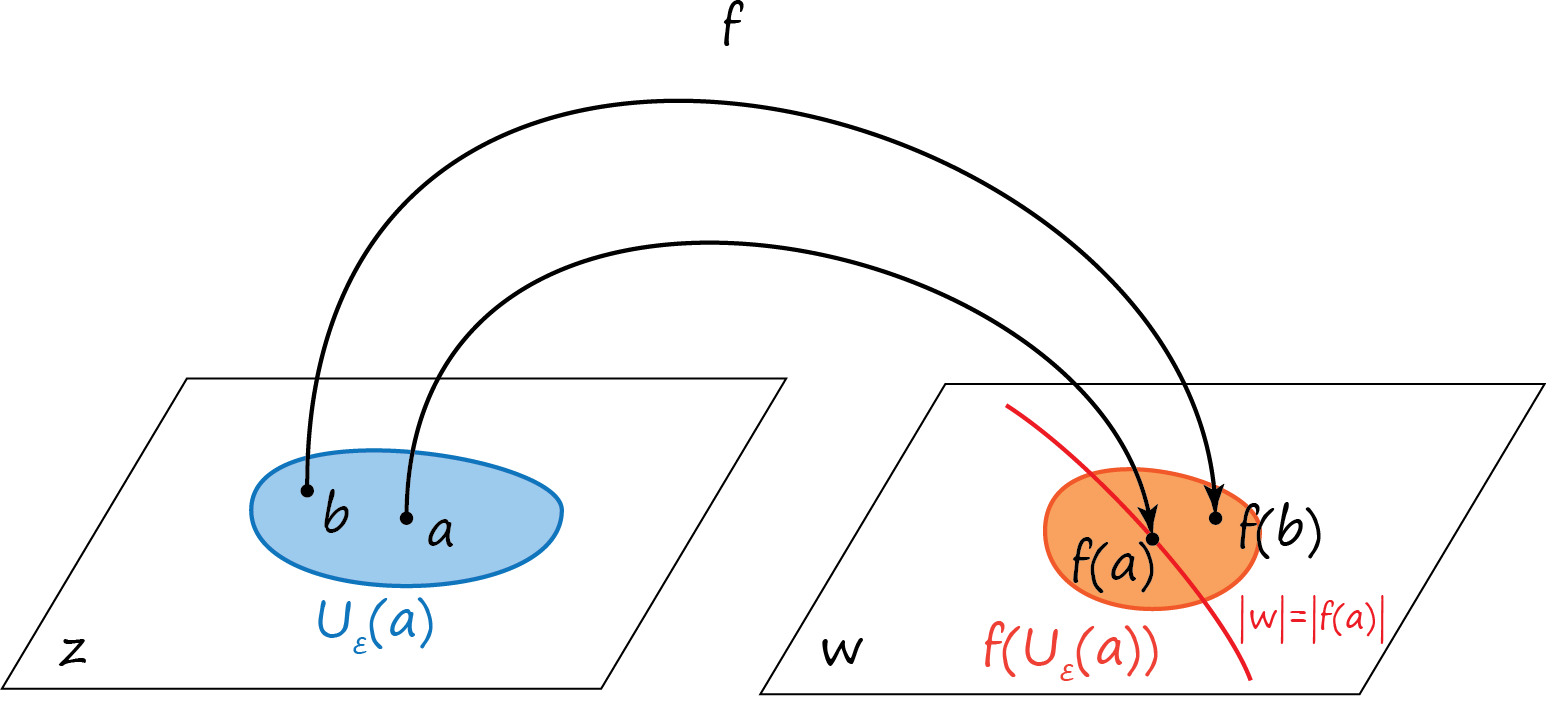
\includegraphics[width=0.6\textwidth]{2016-05-27-analytic-function.png}
\end{figure}

Как мы видим, в окрестности точки \( f(a) \) найдётся точка \( w = f(b) \), для которой \( |f(b)| > |f(a)| \). Но это противоречит нашему допущению о наибольшем значении \( |f(z)| \). Следовательно, \( f(z) = \mathrm{const} \).
\end{document}